\let\negmedspace\undefined
\let\negthickspace\undefined
\documentclass[journal,12pt,onecolumn]{IEEEtran}
\usepackage{cite}
\usepackage{amsmath,amssymb,amsfonts,amsthm}
\usepackage{algorithmic}
\usepackage{graphicx}
\graphicspath{{./figs/}}
\usepackage{textcomp}
\usepackage{xcolor}
\usepackage{txfonts}
\usepackage{listings}
\usepackage{enumitem}
\usepackage{mathtools}
\usepackage{gensymb}
\usepackage{comment}
\usepackage{caption}
\usepackage[breaklinks=true]{hyperref}
\usepackage{tkz-euclide} 
\usepackage{listings}
\usepackage{gvv}                                        
%\def\inputGnumericTable{}                                 
\usepackage[latin1]{inputenc}     
\usepackage{xparse}
\usepackage{color}                                            
\usepackage{array}                                            
\usepackage{longtable}                                       
\usepackage{calc}                                             
\usepackage{multirow}
\usepackage{multicol}
\usepackage{hhline}                                           
\usepackage{ifthen}                                           
\usepackage{lscape}
\usepackage{tabularx}
\usepackage{array}
\usepackage{float}
\newtheorem{theorem}{Theorem}[section]
\newtheorem{problem}{Problem}
\newtheorem{proposition}{Proposition}[section]
\newtheorem{lemma}{Lemma}[section]
\newtheorem{corollary}[theorem]{Corollary}
\newtheorem{example}{Example}[section]
\newtheorem{definition}[problem]{Definition}
\newcommand{\BEQA}{\begin{eqnarray}}
\newcommand{\EEQA}{\end{eqnarray}}
\newcommand{\define}{\stackrel{\triangle}{=}}
\theoremstyle{remark}
\newtheorem{rem}{Remark}

\begin{document}
\title{
ASSIGNMENT 2: GATE 2012 \\
    PH : PHYSICS }
\author{AI25BTECH11035 - Sujal Rajani }
\maketitle
\renewcommand{\thefigure}{\theenumi}
\renewcommand{\thetable}{\theenumi}
\textbf{read the following instruction carefully}
\begin{enumerate}
\item Do not open the seal of the Question Booklet until you are asked to do so by the invigilator.

\item Take out the \textbf{O}ptical \textbf{R}esponse \textbf{S}heet \textbf{(ORS)} from this Question Booklet \textbf{without breaking the seal} and read the instructions printed on the ORS carefully.

\item On the right half of the \textbf{ORS}, using ONLY a \textbf{  black ink ball point pen},  (i) darken the bubble corresponding to your test paper code and the appropriate bubble under each digit of your registration number and  (ii) write your registration number, your name and name of the examination centre and put your signature at the specified location.

\item This Question Booklet contains \textbf{20} pages including blank pages for rough work. After you are permitted to open the seal, please check all pages and report discrepancies, if any, to the invigilator.

\item There are a total of 65 questions carrying 100 marks. All these questions are of objective type.  Each question has only \textbf{one} correct answer. Questions must be answered on the left hand side of the \textbf{ORS} by darkening the appropriate bubble (marked A, B, C, D) using \textbf{ONLY a black ink ball point pen} against the question number. \textbf{For each question darken the bubble of the correct answer} More than one answer bubbled against a question will be treated as an incorrect response.

\item Since bubbles darkened by the black ink ball point pen \textbf{cannot} be erased, candidates should darken the bubbles in the ORS \textbf{very carefully}.

\item Questions Q.1 - Q.25 carry 1 mark each. Questions Q.26 - Q.55 carry 2 marks each. The 2 marks questions include two pairs of common data questions and two pairs of linked answer questions. 
The answer to the second question of the linked answer questions depends on the answer to the first question of the pair. If the first question in the linked pair is wrongly answered or is unattempted, then the answer to the second question in the pair will not be evaluated.

\item Questions Q.56 - Q.65 belong to General Aptitude (GA) section and carry a total of 15 marks.Questions Q.56 - Q.60 carry 1 mark each, and questions Q.61 - Q.65 carry 2 marks each.

\item Unattempted questions will result in zero mark and wrong answers will result in \textbf{NEGATIVE} marks.  For all 1 mark questions, $\tfrac{1}{3}$ mark will be deducted for each wrong answer. For all 2 marks questions, $\tfrac{2}{3}$ mark will be deducted for each wrong answer.  However, in the case of the linked answer question pair, there will be negative marks only for wrong answer to the first question and no negative marks for wrong answer to the second question.

\item Calculator is allowed whereas charts, graph sheets or tables are \textbf{NOT} allowed in the examination hall.

\item Rough work can be done on the question paper itself. Blank pages are provided at the end of the question paper for rough work.

\item Before the start of the examination, write your name and registration number in the space provided below using a black ink ball point pen.
\begin{figure}[H]
    \centering
    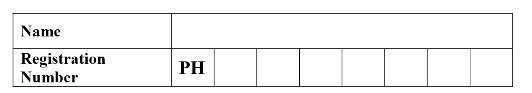
\includegraphics[width = 0.6\columnwidth]{fig/instruction .png}
    \caption*{}
    \label{fig:instruction}
\end{figure}

\end{enumerate}
\newpage
\textbf{Some Useful Constant}

\begin{tabular}{@{}p{0.55\linewidth}l@{}}
Speed of light in free space & $c = 3\times 10^{8}\ \mathrm{m/s}$\\
Boltzmann constant & $k_B = 1.380\times 10^{-23}\ \mathrm{J/K}$\\
Planck's constant & $h = 6.626\times 10^{-34}\ \mathrm{J\cdot s}$\\
Electron charge & $e = 1.602\times 10^{-19}\ \mathrm{C}$\\
Permittivity of free space & $\varepsilon_0 = 8.854\times 10^{-12}\ \mathrm{C^2/(N\cdot m^2)}$\\
Permeability of free space & $\mu_0 = 4\pi\times 10^{-7}\ \mathrm{H/m}$\\
\end{tabular}
\vspace{0.5mm}
NOTE: In numerical problems, the option closest to the correct answer will be given credit.

\vspace{1mm}

\textbf{Q.\ 1 - Q.\ 25 carry one mark each.}


\begin{enumerate}
\item Identify the CORRECT statement for the following vectors
$\vec{a}=3\hat{i}+2\hat{j}$ and $\vec{b}=\hat{i}+2\hat{j}$.
\hfill{\brak{\text{GATE IN 20012}}}
\begin{enumerate}
\item The vectors $\vec{a}$ and $\vec{b}$ are linearly independent
\item The vectors $\vec{a}$ and $\vec{b}$ are linearly dependent
\item The vectors $\vec{a}$ and $\vec{b}$ are orthogonal
\item The vectors $\vec{a}$ and $\vec{b}$ are normalized
\end{enumerate}

\item Two uniform thin rods of equal length, $L$, and masses $M_1$ and $M_2$ are joined together along the length. The moment of inertia of the combined rod of length $2L$ about an axis passing through the mid-point and perpendicular to thelength of the rod is,
\begin{multicols}{2}
\begin{enumerate}
\item $\bigl(M_1+M_2\bigr)\dfrac{L^{2}}{12}$
\item $\bigl(M_1+M_2\bigr)\dfrac{L^{2}}{6}$
\item $\bigl(M_1+M_2\bigr)\dfrac{L^{2}}{3}$
\item $\bigl(M_1+M_2\bigr)\dfrac{L^{2}}{2}$
\end{enumerate}
\end{multicols}

\item The space-time dependence of the electric field of a linearly polarized light in free space is given by$xE_{0}\cos(\omega t-kz)$ where $E_{0}$, $\omega$ and $k$ are the
amplitude, the angular frequency and the wavevector, respectively. The time averaged energy density associated with the electric field is
\begin{multicols}{4}
\begin{enumerate}
\item $\dfrac{1}{4}\varepsilon_{0}E_{0}^{2}$
\item $\dfrac{1}{2}\varepsilon_{0}E_{0}^{2}$
\item $\varepsilon_{0}E_{0}^{2}$
\item $2\varepsilon_{0}E_{0}^{2}$
\end{enumerate}
\end{multicols}

\item If the peak output voltage of a full wave rectifier is 10 V,its d.c.\ voltage is
\begin{multicols}{2}
\begin{enumerate}
\item 10.0 V 
\item 7.07 V
\item 6.36 V 
\item 3.18 V

\end{enumerate}
\end{multicols}


\item A particle of mass $m$ is confined in a two dimensional square well potential of dimension $a$. This potential $V(x,y)$ is given by
$
V(x,y)=0  \text   {for} \  -a < x < a \ \text{and} \ -a < y < a
= \infty  elsewhere
$
The energy of the first excited state for this particle is given by,
\begin{multicols}{4}
\begin{enumerate}
\item $\dfrac{\pi^{2}\hbar^{2}}{ma^{2}}$
\item $\dfrac{2\pi^{2}\hbar^{2}}{ma^{2}}$
\item $\dfrac{5\pi^{2}\hbar^{2}}{2ma^{2}}$
\item $\dfrac{4\pi^{2}\hbar^{2}}{ma^{2}}$
\end{enumerate}
\end{multicols}

\item The isothermal compressibility, $\kappa$ of an ideal gas at temperature $T_{0}$ and volume $V_{0}$, is given by
\begin{multicols}{4}
\begin{enumerate}
\item $-\dfrac{1}{V_{0}}  \dfrac{\partial V}{\partial P} |_{T_{0}}$
\item $\dfrac{1}{V_{0}}  \dfrac{\partial V}{\partial P} |_{T_{0}}$
\item $-V_{0}  \dfrac{\partial P}{\partial V} |_{T_{0}}$
\item $V_{0}  \tfrac{\partial P}{\partial V}|_{T_{0}}$
\end{enumerate}
\end{multicols}

\item The ground state of sodium atom ($^{11}Na$) is a $^{2}S_{1/2}$ state. The difference in energy levels arising in the presence of a weak external magnetic field $B$, given in terms of Bohr magneton, $\mu_{B}$, is
\begin{multicols}{4}
\begin{enumerate}
\item $\mu_{B}B$
\item $2\mu_{B}B$
\item $4\mu_{B}B$
\item $6\mu_{B}B$
\end{enumerate}
\end{multicols}

\item For an ideal Fermi gas in three dimensions, the electron velocity $V_{F}$ at the Fermi surface is related to electron concentration $n$ as,
\begin{multicols}{4}
\begin{enumerate}
\item $V_{F} \propto n^{2/3}$
\item $V_{F} \propto n$
\item $V_{F} \propto n^{1/2}$
\item $V_{F} \propto n^{1/3}$
\end{enumerate}
\end{multicols}

\item Which one of the following sets corresponds to fundamental particles?

\begin{enumerate}
\item proton, electron and neutron
\item proton, electron and photon
\item electron, photon and neutrino
\item quark, electron and meson
\end{enumerate}

\item In case of a Geiger-Muller (GM) counter, which one of the following statements is correct?

\begin{enumerate}
\item Multiplication factor of the detector is of the order of $10^{10}$
\item Type of the particles detected can be identified
\item Energy of the particles detected can be distinguished
\item Operating voltage of the detector is few tens of Volts
\end{enumerate}


\item A plane electromagnetic wave traveling in free space is incident normally on a glass plate of refractive index $3/2$. If there is no absorption by the glass, its reflectivity is
\begin{multicols}{4}
\begin{enumerate}
\item 4\%
\item 16%
\item 20%
\item 50%
\end{enumerate}
\end{multicols}

\item A Ge semiconductor is doped with acceptor impurity concentration of $10^{15}$ atoms/cm$^{3}$. For the given hole mobility of $1800\ \mathrm{cm^{2}/(V\cdot s)}$, the resistivity of this material is
\begin{multicols}{4}
\begin{enumerate}
\item $0.288\ \Omega\mathrm{cm}$
\item $0.694\ \Omega\mathrm{cm}$
\item $3.472\ \Omega\mathrm{cm}$
\item $6.944\ \Omega\mathrm{cm}$
\end{enumerate}
\end{multicols}

\item A classical gas of molecules, each of mass $m$, is in thermal equilibrium at the absolute temperature, $T$. The velocity components of the molecules along the Cartesian axes are $v_x$, $v_y$ and $v_z$. The mean value of $\left( v_x+v_y \right)^{2}$ is
\begin{multicols}{4}
\begin{enumerate}
\item $\dfrac{k_{B}T}{m}$
\item $\dfrac{3}{2}\,\tfrac{k_{B}T}{m}$
\item $\dfrac{1}{2}\,\tfrac{k_{B}T}{m}$
\item $\dfrac{2k_{B}T}{m}$
\end{enumerate}
\end{multicols}

\item In a central force field, the trajectory of a particle of mass $m$ and angular momentum $L$ in plane polar coordinates is given by,

$\dfrac{1}{r} = \dfrac{m}{L^{2}}(1+\varepsilon \cos\theta)$

where, $\varepsilon$ is the eccentricity of the particle motion. Which one of the following choices for $\varepsilon$ gives rise to a parabolic trajectory?
\begin{multicols}{4}
\begin{enumerate}
\item $\varepsilon = 0$
\item $\varepsilon = 1$
\item $0 < \varepsilon < 1$
\item $\varepsilon > 1$
\end{enumerate}
\end{multicols}
\newpage
\item Identify the CORRECT energy band diagram for silicon doped with Arsenic . Here CB,VB,$E_D$ and $E_F$ are conduction band , valence band , impurity level and Fermi level;, respectively
\begin{figure}[H]
    \centering
    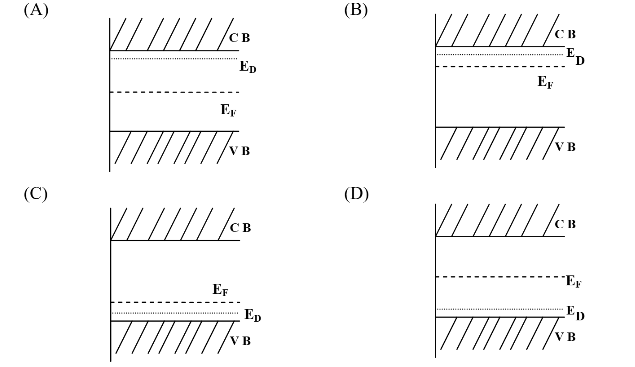
\includegraphics[width = 1\columnwidth]{fig/Q15.png}
    \caption*{}
    \label{fig:Q15}
\end{figure}  

\item The first Stokes line of a rotational Raman spectrum is observed at $12.96\mathrm{cm^{-1}}$. Considering the rigid rotor approximation, the rotational constant is given by
\begin{multicols}{4}
\begin{enumerate}
\item $6.48\ \mathrm{cm^{-1}}$
\item $3.24\ \mathrm{cm^{-1}}$
\item $2.16\ \mathrm{cm^{-1}}$
\item $1.62\ \mathrm{cm^{-1}}$
\end{enumerate}
\end{multicols}

\item The total energy, $E$ of an ideal non-relativistic Fermi gas in three dimensions is given by
$
E \propto \dfrac{N^{5/3}}{V^{2/3}}
$
where $N$ is the number of particles and $V$ is the volume of the gas. Identify the \textsc{correct} equation of state ($P$ being the pressure),
\begin{multicols}{4}
\begin{enumerate}
\item $PV = \dfrac{1}{3}E$
\item $PV = \dfrac{2}{3}E$
\item $PV = E$
\item $PV = \dfrac{5}{3}E$
\end{enumerate}
\end{multicols}

\item Consider the wavefunction $\Psi = \psi(\vec{r}_1, \vec{r}_2)\chi_s$ for a fermionic system consisting of two spin-half particles. The spatial part of the wavefunction is given by,
$
\psi(\vec{r}_1, \vec{r}_2) = \frac{1}{\sqrt{2}}  \phi_{1}(\vec{r}_1)\phi_{2}(\vec{r}_2) + \phi_{2}(\vec{r}_1)\phi_{1}(\vec{r}_2) $
where $\phi_1$ and $\phi_2$ are single particle states. The spin part $\chi_s$ of the wavefunction with spin states $\alpha$ $(+{1}/{2})$ and $\beta$ $(-{1}/{2})$ should be
\begin{multicols}{4}
\begin{enumerate}
\item $\tfrac{1}{\sqrt{2}} (\alpha\beta + \beta\alpha)$
\item $\tfrac{1}{\sqrt{2}} (\alpha\beta - \beta\alpha)$
\item $\alpha\alpha$
\item $\beta\beta$
\end{enumerate}
\end{multicols}

\item The electric and the magnetic fields $\vec{E}(z,t)$ and $\vec{B}(z,t)$, respectively corresponding to the scalar potential $\phi(z,t)=0$ and vector potential $\vec{A}(z,t)=\hat{i}\,t\,z$ are
\begin{multicols}{2}
\begin{enumerate}
\item $\vec{E} = \hat{i}z and \vec{B} = -j\,t$
\item $\vec{E} = \hat{i}z and \vec{B} = j\,t$
\item $\vec{E} = -\hat{i}z and \vec{B} = -j\,t$
\item $\vec{E} = -\hat{i}z and  \vec{B} = j\,t$
\end{enumerate}
\end{multicols}
\item Consider the folowing OP-AMP circuit
\begin{figure}[H]
    \centering
    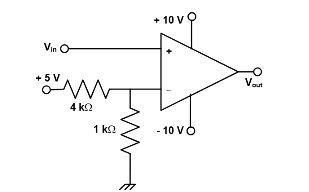
\includegraphics[width = 0.5\columnwidth]{fig/Q20(1).png}
    \caption*{}
    \label{fig:Q20(1)}
\end{figure}
Which one of the following correctly represent the output $V_{out}$
 corresponding to the input  $V_{in}$ ?
 \begin{figure}[H]
    \centering
    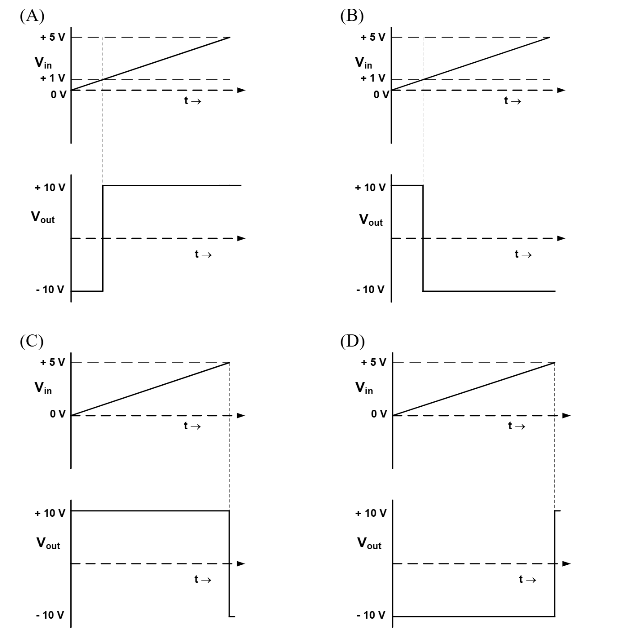
\includegraphics[width = 0.7\columnwidth]{fig/Q20(2).png}
    \caption*{}
    \label{fig:Q20(2)}
\end{figure}
\item Deuteron has only one bound state with spin parity $1^+$, isospin 0 and electric quadrupole moment $0.286\, efm^2$ . These data suggest that the nuclear forces are having
\begin{enumerate}
    \item only spin and isospin dependence
    \item no spin dependence and no tensor components
    \item spin dependence and no tensor components 
    \item spin dependence along with tensor components
\end{enumerate}


\item A particle of unit mass moves along the $x$-axis under the influence of a potential,$V(x)=x(x-2)^{2}$. The particle is found to be in stable equilibrium at the point $x=2$.The time period of oscillation of the particle is
\begin{multicols}{4}
\begin{enumerate}
\item $\dfrac{\pi}{2}$
\item $\pi$
\item $\dfrac{3\pi}{2}$
\item $2\pi$
\end{enumerate}
\end{multicols}

\item Which one of the following CANNOT be explained by considering a harmonic approximation
for the lattice vibrations in solids?
\begin{multicols}{2}
\begin{enumerate}
\item Debye $T^{3}$ law
\item Dulong-Petits law
\item Optical branches in lattices
\item Thermal expansion
\end{enumerate}
\end{multicols}

\item A particle is constrained to move in a truncated harmonic potential well ($x>0$) as shown.Which one of the following statements is CORRECT?

\begin{figure}[H]
    \centering
    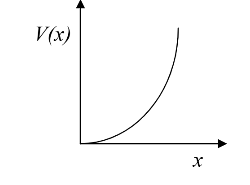
\includegraphics[width = 0.5\columnwidth]{fig/Q24.png}
    \caption*{}
    \label{fig:Q24}
\end{figure}
\begin{enumerate}
\item The parity of the first excited state is even
\item The parity of the ground state is even
\item The ground state energy is $\tfrac{1}{2}\hbar\omega$
\item The first excited state energy is $\tfrac{7}{2}\hbar\omega$
\end{enumerate}


\item The number of independent components of the symmetric tensor $A_{ij}$ with indices
$i,j=1,2,3$ is
\begin{multicols}{4}
\begin{enumerate}
\item 1
\item 3
\item 6
\item 9
\end{enumerate}
\end{multicols}


\subsection*{Q.\ 26 to Q.\ 55 carry two marks each.}

\item Consider a system in the unperturbed state described by the Hamiltonian
$H_{0}=\begin{pmatrix}1&0\\[2pt]0&1\end{pmatrix}$. The system is subjected to a
perturbation of the form
$H'=\begin{pmatrix}\delta&\delta\\[2pt]\delta&\delta\end{pmatrix}$, where
$\delta\ll 1$. The energy eigenvalues of the perturbed system using the first
order perturbation approximation are
\begin{multicols}{2}
\begin{enumerate}
\item $1 \text{ and } (1+2\delta)$
\item $(1+\delta) \text{ and } (1-\delta)$
\item $(1+2\delta) \text{ and } (1-2\delta)$
\item $(1+\delta) \text{ and } (1-2\delta)$
\end{enumerate}
\end{multicols}
\item Inverse susceptibility $(1/\chi)$ as a function of temperature, $T$ for a material undergoing paramagnetic to ferromagnetic transition is given in the figure, where O is the origin. The values of the Curie constant, $C$, and the Weiss molecular field constant, $\lambda$, in CGS units, are
\begin{figure}[H]
    \centering
    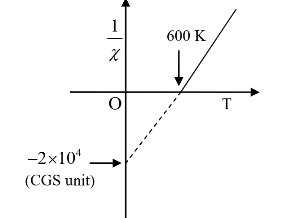
\includegraphics[width = 0.5\columnwidth]{fig/Q27.png}
    \caption*{}
    \label{fig:Q27}
    \end{figure}
\begin{multicols}{2}
\begin{enumerate}
\item $C=5\times 10^{-5} \lambda=3\times 10^{-2}$
\item $C=3\times 10^{-2} \lambda=5\times 10^{-5}$
\item $C=3\times 10^{-2} \lambda=2\times 10^{4}$
\item $C=2\times 10^{4} \lambda=3\times 10^{-2}$
\end{enumerate}
\end{multicols}

\item A plane polarized electromagnetic wave in free space at time $t=0$ is given by$\vec{E}(x,z)=10\hat{j}\,\exp\bigl[i(6x+8z)\bigr].$The magnetic field $\vec{B}(x,z,t)$ is given by

\begin{enumerate}
\item $ \vec{B}(x,z,t) = \dfrac{1}{c}\,(6\hat{k}-8\hat{i})\exp\bigl[i(6x+8z-10ct)\bigr]$
\item $ \vec{B}(x,z,t) =\dfrac{1}{c}\,(6\hat{k}+8\hat{i})\exp\bigl[i(6x+8z-10ct)\bigr]$
\item $ \vec{B}(x,z,t) =\dfrac{1}{c}\,(6\hat{k}-8\hat{i})\exp\bigl[i(6x+8z-ct)\bigr]$
\item $\vec{B}(x,z,t) =\dfrac{1}{c}(6\hat{k}+8\hat{i})\exp\bigl[i(6x+8z+ct)\bigr]$
\end{enumerate}


\item The eigenvalues of the matrix
$
\begin{pmatrix}
0 & 1 & 0\\[4pt]
1 & 0 & 1\\[4pt]
0 & 1 & 0
\end{pmatrix}
$
are
\begin{multicols}{4}
\begin{enumerate}
\item $0,\,1,\,1$
\item $0,\,-\sqrt{2},\,\sqrt{2}$
\item $\dfrac{1}{\sqrt{2}},\dfrac{1}{\sqrt{2}},\,0$
\item $\sqrt{2},\sqrt{2},0$
\end{enumerate}
\end{multicols}

\item Match the typical spectroscopic regions specified in Group I with the corresponding type of transitions in Group II.
\begin{center}
\begin{tabular}{@{}p{0.45\linewidth}p{0.45\linewidth}@{}}
\textbf{Group I} & \textbf{Group II} \\[4pt]
(P) Infra-red region & (i) electronic transitions involving valence electrons \\[4pt]
(Q) Ultraviolet-visible region & (ii) nuclear transitions \\[4pt]
(R) X-ray region & (iii) vibrational transition of molecules\\[4pt]]
(s) $\gamma$ ray region & (iv) transitions involving inner shell electrons

\end{tabular}
\end{center}
\begin{enumerate}
\begin{multicols}{2}
     \item (P,i);(Q,iii);(R,ii);(S,iv)
    \item (P,ii);(Q,iv);(R,i);(S,iii)
    \item (P,iii);(Q,i);(R,iv);(S,ii)
    \item (P,iv);(Q,iii);(R,ii);(S,iii)
\end{multicols}
   
\end{enumerate}


\item In the following circuit, for the output voltage to be $V_{o}=(-\,V_{1}\;|\;V_{2}/2)$, the ratio $R_1/R_2$ is
\begin{figure}[H]
    \centering
    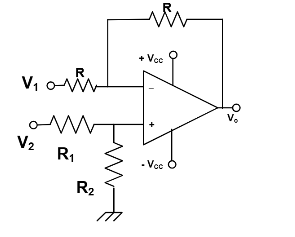
\includegraphics[width = 0.6\columnwidth]{fig/Q31.png}
    \caption*{}
    \label{fig:Q31}
\end{figure}

\begin{multicols}{4}
\begin{enumerate}
\item 1/2
\item 1
\item 2
\item 3
\end{enumerate}
\end{multicols}

\item The terms $\{j_{1},j_{2}\}$ arising from $2s^{1}3d^{1}$ electronic configuration in $j$-$j$ coupling scheme are
\begin{multicols}{2}
\begin{enumerate}
\item $\bigl\{\dfrac{1}{2},\dfrac{3}{2}\bigr\}_{2,1} and \bigl\{\dfrac{1}{2},\dfrac{5}{2}\bigr\}_{3,2}$
\item $\bigl\{\dfrac{1}{2},\dfrac{1}{2}\bigr\}_{1,0}  and  \bigl\{\dfrac{1}{2},\dfrac{3}{2}\bigr\}_{2,1}$
\item $\bigl\{\dfrac{1}{2},\dfrac{1}{2}\bigr\}_{1,0} and   \bigl\{\dfrac{1}{2},\dfrac{5}{2}\bigr\}_{3,2}$
\item $\bigl\{\dfrac{3}{2},\dfrac{1}{2}\bigr\}_{2,1} and \bigl\{\dfrac{1}{2},\dfrac{5}{2}\bigr\}_{3,2}$
\end{enumerate}
\end{multicols}

\item In the following circuit, the voltage drop across the ideal diode in forward bias condition is $0.7\ \mathrm{V}$. 
\begin{figure}[H]
    \centering
    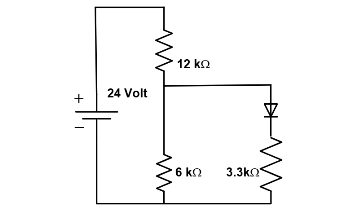
\includegraphics[width = 0.6\columnwidth]{fig/Q33.png}
    \caption*{}
    \label{fig:Q33}
\end{figure}

The current passing through the diode is
\begin{multicols}{4}
\begin{enumerate}
\item $0.5\ \mathrm{mA}$
\item $1.0\ \mathrm{mA}$
\item $1.5\ \mathrm{mA}$
\item $2.0\ \mathrm{mA}$
\end{enumerate}
\end{multicols}

\item Choose the CORRECT statement from the following.
\begin{multicols}{2}
\begin{enumerate}
\item Neutron interacts through electromagnetic interaction
\item Electron does not interact through weak interaction
\item Neutrino interacts through weak and electromagnetic interaction
\item Quark interacts through strong interaction but not through weak interaction
\end{enumerate}
\end{multicols}

\item A rod of proper length $l_{0}$ oriented parallel to the $x$-axis moves with speed $2c/3$ along the $x$-axis in the $S$-frame, where $c$ is the speed of light in free space. The observer is also moving along the $x$-axis with speed $c/2$ with respect to the $S$-frame. The length of the rod as measured by the observer is
\begin{multicols}{4}
\begin{enumerate}
\item $0.35\,l_{0}$
\item $0.48\,l_{0}$
\item $0.87\,l_{0}$
\item $0.97\,l_{0}$
\end{enumerate}
\end{multicols}

\item parameter $a_{c}$ undergoes transition into a tetragonal structure with lattice parameters $a_{t}=b_{t}=\sqrt{2}\,a_{c}$ and $c_{t}=2a_{c}$ below a certain temperature. The ratio of the interplanar spacings of $(1\ 0\ 1)$ planes for the cubic and the tetragonal structures is
\begin{multicols}{2}
\begin{enumerate}
\item $\sqrt{\tfrac{1}{6}}$
\item $\tfrac{1}{6}$
\item $\sqrt{\tfrac{3}{8}}$
\item $\tfrac{3}{8}$
\end{enumerate}
\end{multicols}

\item Consider the following circuit in which the current gain $\beta_{dc}$ of the transistor is $100$.
\begin{figure}[H]
    \centering
    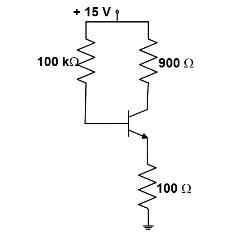
\includegraphics[width = 0.3\columnwidth]{fig/Q37(1).png}
    \caption*{}
    \label{fig:Q37(1)}
    \end{figure}
    which one of the following correctly represents the load line (collector current $I_c$ with respect to collector -emitter voltage $V_{CE}$)  Q-point of this circuit ?
    \begin{figure}[H]
    \centering
    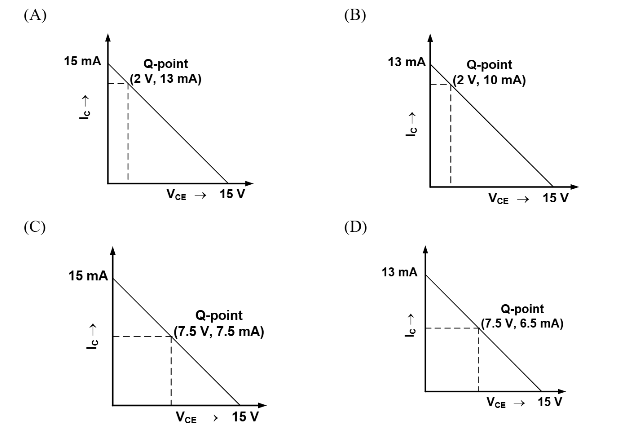
\includegraphics[width = 1\columnwidth]{fig/Q37(2).png}
    \caption*{}
    \label{fig:Q37(2)}
    \end{figure}
\item Consider a system whose three energy levels are given by $0$, $\varepsilon$ and $2\varepsilon$. The energy level $\varepsilon$ is two-fold degenerate and the other two are non-degenerate. The partition function of the system with $\beta = \frac{1}{k_{B}T}$ is given by
\begin{multicols}{2}
\begin{enumerate}
\item $1 + 2e^{-\beta\varepsilon}$
\item $2e^{-\beta\varepsilon} + e^{-2\beta\varepsilon}$
\item $(1 + e^{\beta\varepsilon})^{2}$
\item $1 + e^{\beta\varepsilon} + e^{2\beta\varepsilon}$
\end{enumerate}
\end{multicols}

\item Two infinitely extended homogeneous isotropic dielectric media (medium-1 and medium-2) with dielectric constants $\frac{\varepsilon_{1}}{\varepsilon_{0}} = 2$ and $\frac{\varepsilon_{2}}{\varepsilon_{0}} = 5$, respectively, meet at the $z=0$ plane as shown in the figure. A uniform electric field exists everywhere. For $z \geq 0$, the electric field is given by $\vec{E}_{1} = 2\hat{i} - 3\hat{j} + 5\hat{k}$. The interface separating the two media is charge free.

The electric displacement vector in the medium-2 is given by
\begin{figure}[H]
    \centering
    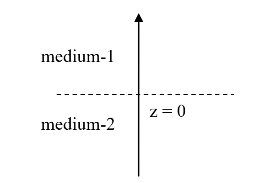
\includegraphics[width = 0.35\columnwidth]{fig/Q39.png}
    \caption*{}
    \label{fig:Q39}
\end{figure}
\begin{multicols}{2}
\begin{enumerate}
\item $\vec{D}_{2} = \varepsilon_{0}[10\hat{i} + 15\hat{j} + 10\hat{k}]$
\item $\vec{D}_{2} = \varepsilon_{0}[10\hat{i} - 15\hat{j} + 10\hat{k}]$
\item $\vec{D}_{2} = \varepsilon_{0}[4\hat{i} - 6\hat{j} + 10\hat{k}]$
\item $\vec{D}_{2} = \varepsilon_{0}[4\hat{i} + 6\hat{j} + 10\hat{k}]$
\end{enumerate}
\end{multicols}
\item  The ground state wavefunction for the hydrogen atom is given by $\psi_{100} = \frac{1}{\sqrt{4\pi}} \left( \frac{1}{a_{0}} \right)^{3/2} e^{-r/a_{0}},$ where $a_{0}$ is the Bohr radius.
The plot of the radial probability density, $P(r)$ for the hydrogen atom in the ground state is

\begin{figure}[H]
    \centering
    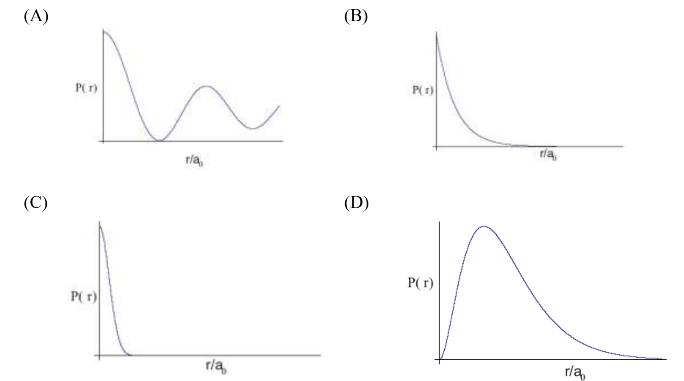
\includegraphics[width = 0.9\columnwidth]{fig/Q40.png}
    \caption*{}
    \label{fig:Q40}
\end{figure}


\item Total binding energies of O$^{15}$, O$^{16}$ and O$^{17}$ are $111.96\ MeV$, $127.62\ MeV$ and $131.76\ MeV$, respectively. The energy gap between $1p_{1/2}$ and $1d_{5/2}$ neutron shells for the nuclei whose mass number is close to $16$, is
\begin{multicols}{4}
\begin{enumerate}
\item $4.1\ MeV$
\item $11.5\ MeV$
\item $15.7\ MeV$
\item $19.8\ MeV$
\end{enumerate}
\end{multicols}

\item A particle of mass $m$ is attached to a fixed point O by a weightless inextensible string of length $a$. It is rotating under gravity as shown in the figure. The Lagrangian of the particle is $ L(\theta,\phi) = \frac{1}{2} m a^{2} \left( \dot{\theta}^{2} + \sin^{2}\theta\,\dot{\phi}^{2} \right) - m g a \cos\theta $
where $\theta$ and $\phi$ are the polar angles.

\begin{figure}[H]
    \centering
    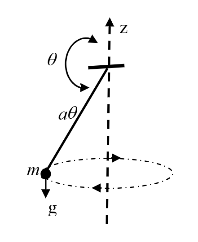
\includegraphics[width=0.35\columnwidth]{fig/Q42.png}
    \label{fig:Q42}
\end{figure}

The Hamiltonian of the particle is
\begin{multicols}{2}
\begin{enumerate}
\item $H = \frac{1}{2 m a^{2}}\left( p_{\theta}^{2} + \frac{p_{\phi}^{2}}{\sin^{2}\theta} \right) - m g a \cos\theta$
\item $H = \frac{1}{2 m a^{2}}\left( p_{\theta}^{2} + \frac{p_{\phi}^{2}}{\sin^{2}\theta} \right) + m g a \cos\theta$
\item $H = \frac{1}{2 m a^{2}}\left( p_{\theta}^{2} + p_{\phi}^{2} \right) - m g a \cos\theta$
\item $H = \frac{1}{2 m a^{2}}\left( p_{\theta}^{2} + p_{\phi}^{2} \right) + m g a \cos\theta$
\end{enumerate}
\end{multicols}

\item Given $\vec{F} = \vec{r} \times \vec{B}$, where $\vec{B} = B_{0}(\hat{i} + \hat{j} + \hat{k})$ is a constant vector and $\vec{r}$ is the position vector. The value of $\oint_{C} \vec{F} \cdot d\vec{r}$, where $C$ is a circle of unit radius centered at the origin, is
\begin{figure}[H]
    \centering
    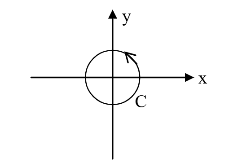
\includegraphics[width=0.25\columnwidth]{fig/Q43.png}
    \label{fig:Q43}
\end{figure}
\begin{multicols}{4}
\begin{enumerate}
\item $0$
\item $2\pi B_{0}$
\item $-2\pi B_{0}$
\item $1$
\end{enumerate}
\end{multicols}

\item The value of the integral $\oint_{C} e^{1/z} dz$, using the contour $C$ of a circle with unit radius $|z| = 1$, is
\begin{multicols}{4}
\begin{enumerate}
\item $0$
\item $1 - 2\pi i$
\item $1 + 2\pi i$
\item $2\pi i$
\end{enumerate}
\end{multicols}

\item A paramagnetic system consisting of $N$ spin-half particles, is placed in an external magnetic field. It is found that $N/2$ spins are aligned parallel and the remaining $N/2$ spins are aligned antiparallel to the magnetic field. The statistical entropy of the system is
\begin{multicols}{2}
\begin{enumerate}
\item $ 2 N k_{B} \ln 2 $
    \item $ \dfrac{N}{2} k_{B} \ln 2 $
    \item  $\dfrac{3N}{2} k_{B} \ln 2 $
    \item  $N k_{B} \ln 2 $
\end{enumerate}
\end{multicols}

\item The equilibrium vibration frequency for an oscillator is observed at $ 2990 \ \mathrm{cm^{-1}} $. The ratio of the frequencies corresponding to the first and the fundamental spectral lines is  1.96 . Considering the oscillator to be anharmonic, the anharmonicity constant is:
\begin{multicols}{4}
\begin{enumerate}
    \item 0.005
    \item 0.02
    \item 0.05
     \item 0.1
\end{enumerate}
\end{multicols}
    


\item At a certain temperature  T , the average speed of nitrogen molecules in air is found to be $ 400 \ \mathrm{m/s} $. The most probable and the root mean square speeds of the molecules are, respectively:
\begin{multicols}{2}
\begin{enumerate}
    \item 355 m/s, 434 m/s
    \item 820 m/s, 917 m/s
    \item 152 m/s, 301 m/s
    \item 422 m/s, 600 m/s
\end{enumerate}
\end{multicols}
\textbf{Common Data for Questions 48 and 49:}
 The wavefunction of a particle moving in free space is given by,
$ \psi = e^{ikx} + 2 e^{-ikx} $
\item The energy of the particle is:
\begin{multicols}{2}
\begin{enumerate}
    \item $\dfrac{5\hbar^2 k^2}{2m} $
    \item $ \dfrac{3\hbar^2 k^2}{4m} $
    \item $ \dfrac{\hbar^2 k^2}{2m} $
    \item $ \dfrac{\hbar^2 k^2}{m} $
\end{enumerate}
\end{multicols}

\item The probability current density for the real part of the wavefunction is:
\begin{multicols}{2}
\begin{enumerate}
    \item 1
    \item $ \dfrac{\hbar k}{m} $
    \item $ \dfrac{\hbar k}{2m} $
    \item 0
\end{enumerate}
\end{multicols}
 \textbf{Common Data for Questions 50 and 51:} \\

The dispersion relation for a one-dimensional monatomic crystal with lattice spacing $a$, which interacts via nearest neighbour harmonic potential is given by
$
\omega = A \biggl| \sin \frac{Ka}{2} \biggr|,
$
where $A$ is a constant of appropriate unit.

\item The group velocity at the boundary of the first Brillouin zone is:
\begin{multicols}{4}
\begin{enumerate}
    \item 0
    \item 1
    \item $\sqrt{\frac{Aa^2}{2}}$
    \item $\frac{1}{2} \sqrt{\frac{Aa^2}{2}}$
\end{enumerate}
\end{multicols}

\item The force constant between the nearest neighbour of the lattice is ($M$ is the mass of the atom):
\begin{multicols}{4}
\begin{enumerate}
    \item $\frac{MA^2}{4}$
    \item $\frac{MA^2}{2}$
    \item $MA^2$
    \item $2MA^2$
\end{enumerate}
\end{multicols}

\textbf{Statement for Linked Answer Questions 52 and 53: }
In a hydrogen atom, consider that the electronic charge is uniformly distributed in a spherical volume of radius  a (= 0.5x $10^{-10}$ m) around the proton. The atom is placed in a uniform electric field E = 30 x $10^5$ V/m.
Assume that the spherical distribution of the negative charge remains undistorted under the electric field. 
\item In the equilibrium condition, the separation between the positive and the negative charge centers is:
\begin{multicols}{4}
\begin{enumerate}
    \item $ 8.66 \times 10^{-16} $
    \item $ 2.60 \times 10^{-15} $
    \item $ 2.60 \times 10^{-16} $
    \item $ 8.66 \times 10^{-15} $
\end{enumerate}
\end{multicols}
\item The polarizability of the hydrogen atom in unit of ($\mathrm{C^2 m/N}$) is:
\begin{multicols}{4}
\begin{enumerate}
    \item $ 2.0 \times 10^{-40} $
    \item $ 1.4 \times 10^{-41} $
    \item $ 1.4 \times 10^{-40} $
    \item $ 2.0 \times 10^{-39} $
\end{enumerate}
\end{multicols}
\textbf{Statement for Linked Answer Questions 54 and 55:}

A particle of mass $m$ slides under the gravity without friction along the parabolic path $ y = ax^2 $ as shown in the figure. Here $a$ is a constant.
\begin{figure}[H]
    \centering
    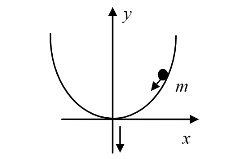
\includegraphics[width = 0.3\columnwidth]{fig/Q54 TO Q55.png}
    \caption*{}
    \label{fig:Q54 TO Q55.png}
\end{figure}
\item The Lagrangian for this particle is given by,
\begin{multicols}{2}
\begin{enumerate}[label=\Alph*)]
    \item $ L = \dfrac{1}{2} m\dot{x}^2 - mgax^2 $
    \item $ L = \dfrac{1}{2} m (1 + 4a^2 x^2) \dot{x}^2 - mgax^2 $
    \item $ L = \dfrac{1}{2} m\dot{x}^2 + mgax^2 $
    \item $ L = \dfrac{1}{2} m (1 + 4a^2 x^2) \dot{x}^2 + mgax^2 $
\end{enumerate}
\end{multicols}

\item The Lagrange's equation of motion of the particle is:
\begin{multicols}{2}
\begin{enumerate}[label=\Alph*)]
    \item $ \ddot{x} = 2gax $
    \item $ m(1 + 4a^2 x^2) \ddot{x} = -2mgax - 4ma^2 x\dot{x}^2 $
    \item $ m(1 + 4a^2 x^2) \ddot{x} = 2mgax + 4ma^2 x\dot{x}^2 $
    \item $ \ddot{x} = -2gax $
\end{enumerate}
\end{multicols}
\textbf{General Aptitude (GA) Questions}

Q.56 -- Q.60 carry one mark each.

\item Choose the grammatically \textbf{INCORRECT} sentence:

\begin{enumerate}
    \item They gave us the money back less the service charges of Three Hundred rupees.
    \item This country expenditure is not less than that of Bangladesh.
    \item The committee initially asked for a funding of Fifty Lakh rupees, but later settled for a lesser sum.
    \item This country's expenditure on educational reforms is very less.
\end{enumerate}


\item Which one of the following options is the closest in meaning to the word given below? 
Mitigate
\begin{multicols}{4}
\begin{enumerate}
    \item Diminish
    \item Divulge
    \item Dedicate
    \item Denote
\end{enumerate}
\end{multicols}

\item Choose the most appropriate alternative from the options given below to complete the following sentence: 
\textbf{Despite several \_\_\_\_\_\_\_\_ the mission succeeded in its attempt to resolve the conflict.}
\begin{multicols}{4}
\begin{enumerate}[label=\Alph*)]
    \item attempts
    \item setbacks
    \item meetings
    \item delegations
\end{enumerate}
\end{multicols}

\item The cost function for a product in a firm is given by $ 5q^2 $, where $q$ is the amount of production. The firm can sell the product at a market price of  $50$ per unit. The number of units to be produced by the firm such that the profit is maximized is:
\begin{multicols}{4}
\begin{enumerate}
    \item 5
    \item 10
    \item 15
    \item 25
\end{enumerate}
\end{multicols}

\item Choose the most appropriate alternative from the options given below to complete the following sentence: 
\textit{Suresh's dog is the one \_\_\_\_\_\_\_\_ was hurt in the stampede.}
\begin{multicols}{2}
\begin{enumerate}[label=\Alph*)]
    \item that
    \item which
    \item who
    \item whom
\end{enumerate}
\end{multicols}

Q.61 -- Q.65 carry two marks each.

\item Which of the following assertions are \textbf{CORRECT}? 
P: Adding 7 to each entry in a list adds 7 to the mean of the list 
Q: Adding 7 to each entry in a list adds 7 to the standard deviation of the list 
R: Doubling each entry in a list doubles the mean of the list 
S: Doubling each entry in a list leaves the standard deviation of the list unchanged
\begin{multicols}{4}
\begin{enumerate}
    \item P, Q
    \item Q, R
    \item P, R
    \item R, S
\end{enumerate}
\end{multicols}
\item An automobile plant contracted to buy shock absorbers from two suppliers X and Y. X supplies $60\%$ and Y supplies $40\%$ of the shock absorbers. All shock absorbers are subjected to a quality test. The ones that pass the quality test are considered reliable. Of X's shock absorbers, $96\%$ are reliable. Of Y's shock absorbers, $72\%$ are reliable. \\

The probability that a randomly chosen shock absorber, which is found to be reliable, is made by Y is:
\begin{multicols}{4}
\begin{enumerate}
    \item 0.288
    \item 0.334
    \item 0.667
    \item 0.720
\end{enumerate}
\end{multicols}

\item A political party orders an arch for the entrance to the ground in which the annual convention is being held. The profile of the arch follows the equation $y = 2x - 0.1x^2$ where $y$ is the height of the arch in meters. The maximum possible height of the arch is:
\begin{multicols}{2}
\begin{enumerate}[label=\Alph*)]
    \item 8 meters
    \item 10 meters
    \item 12 meters
    \item 14 meters
\end{enumerate}
\end{multicols}

\item \textbf{Wanted Temporary, Part-time persons for the post of Field Interviewer to conduct personal interviews to collect and collate economic data. Requirements: High School-pass, must be available for Day, Evening and Saturday work. Transportation paid, expenses reimbursed.} 

Which one of the following is the best inference from the above advertisement?

\begin{enumerate}
    \item Gender-discriminatory
    \item Xenophobic
    \item Not designed to make the post attractive
    \item Not gender-discriminatory
\end{enumerate}


\item Given the sequence of terms, AD \quad CG \quad FK \quad JP, the next term is:
\begin{multicols}{4}
\begin{enumerate}
    \item OV
    \item OW
    \item PV
    \item PW
\end{enumerate}
\end{multicols}


\section*{END OF THE QUESTION PAPER}
\end{enumerate}

 




\end{document}